\subsection{Rollout Drift and Likelihood Across the Model Ladder}\label{app:ladderfid}

All \TestHalfN{} mid-training world-model checkpoints pass the same short-horizon quality thresholds as the full-budget runs (\TestHalfPass{} of \TestHalfN{}), as one-month structural changed-tile F1 spans \TestHalfFOneMin{} to \TestHalfFOneMax{} with \RollA-month median relative errors of \TestHalfPopMin{}--\TestHalfPopMax{} on population and \TestHalfFundsMin{}--\TestHalfFundsMax{} on municipal funds (even at month \RollA{}, static start-state copying incurs just \TestCopyPop{} relative population error). On the primary checkpoint at month \Horizon{}, the seven non-\HorBestOverlay{} spatial overlays span \HorRestMin{} to \HorRestMax{} times copy error (vs.\ \HorEngMin{}--\HorEngMax{} for cross-seed engine replays, with fire coverage at \HorFireEmu{} vs.\ \HorFireEng{}). \ifHorizonDone\HorLadderSentence\fi{} \ifLogVerdDone\LogVerdLadderSentence\fi{}

\subsection{Sixfold Extended One-Step Training Control}\label{app:extended}

To test whether the primary two-epoch checkpoint's \Horizon-month rollout drift, planning false acceptance, and downstream discovery shortfall stem simply from early stopping on the \TrainTransitions-transition store, we trained a single-seed \SizeM{} full-data one-step world model from scratch for \ExtTrSamples{} examples (\ExtTrEpochs{} passes over \TrainTransitions{} transitions under a stretched cosine schedule, final SHA-256 prefix \texttt{\ExtTrSha}; Table~\ref{tab:extended}), evaluating milestones at \HpSamplesOs{}-example intervals. Held-out variational log-likelihood improves monotonically across all six milestones from \ExtTrBaseTestElbo{} (primary two-epoch checkpoint) to \ExtTrTestElbo{} nats on the test split (\ExtTrDevElbo{} on development; terminal relative loss slope \ExtTrLossSlopePct{} per cent per hundred thousand examples, gaining \ExtTrLastTwoElboGain{} nats over the final two epochs as latent KL rises from \ExtTrKlStart{} to \ExtTrKlEnd{} nats), while \RollA-month median relative funds error drops from \ExtTrFirstFunds{} at two epochs (\TestMainFunds{} on the primary schedule) to \ExtTrTestFunds{} and one-month structural F1 reaches \ExtTrTestFOne{} \ci{\ExtTrTestFOneCI}. By contrast, \Horizon-month mean spatial-overlay copy ratio worsens monotonically from \ExtTrFirstMeanOv{} to \ExtTrMeanOv{} (\ExtTrGeCopy{} of \HorOverlays{} overlays exceeding copy error, vs.\ \ExtTrSeedGeMin{}--\ExtTrSeedGeMax{} across three two-epoch seeds) and open-loop powered-zone error climbs to \ExtTrPowMae{} tiles (\ExtTrSeedPowMin{}--\ExtTrSeedPowMax{} across three two-epoch seeds, and \ExtTrTrainPowBase{} to \ExtTrTrainPow{} on training cities), shifting open-loop spatial rollouts pessimistic. Across the six milestones on all \AllCities{} held-out cities (\AllInstances{} instances), single-plan ($B ={}$\Bp{0}) excess false acceptance remains strictly positive through \ExtTrMileEightEpochs{} epochs (\ExtTrMileEightSamples{} examples, \ExtTrMileEightExcess{} \ci{\ExtTrMileEightExcessCI}) before crossing zero at \ExtTrMileTenEpochs{}--\ExtTrEpochs{} epochs (\ExtTrMileTenExcess{} \ci{\ExtTrMileTenExcessCI} and \ExtTrRandOneAllExcess{} \ci{\ExtTrRandOneAllExcessCI}) as model self-acceptance falls from \ExtTrMileTwoJudgeAcc{} to \ExtTrRandOneAllJudgeAcc{} and false rejection climbs from \ExtTrMileTwoFalseRej{} to \ExtTrRandOneAllFalseRej{} (on \emph{treasury}, single-plan excess sits at \ExtTrRandOneAllTreasExcess{} \ci{\ExtTrRandOneAllTreasExcessCI} with \ExtTrRandOneAllTreasFalseRej{} false rejection). Replaying Figure~\ref{fig:env}'s coal-plant demolition blackout plan on CPU confirms that the \ExtTrEpochs-epoch model still passes \ExtTrFigOnePass{} of \FigOneK{} rollouts (matching the primary checkpoint), whereas across Figure~\ref{fig:gallery}'s \GalPairs{} showcase plans model acceptance falls monotonically from \ExtTrGalStartAcc{} of \GalPairs{} at two epochs to \ExtTrGalEndAcc{} of \GalPairs{} at \ExtTrEpochs{} epochs (both remaining acceptances on \emph{power}). At \ExtTrEpochs{} epochs across all \AllCities{} cities, raw false acceptance falls to \ExtTrRandOneAllHack{} at \Bp{0}, \ExtTrRandThouAllHack{} under \Bp{3} random shooting (excess \ExtTrRandThouAllExcess{} \ci{\ExtTrRandThouAllExcessCI}; false rejection \ExtTrRandThouAllFalseRej{}), and \ExtTrAdThouAllHack{} under \Bp{3} adaptive CEM (excess \ExtTrAdThouAllExcess{} \ci{\ExtTrAdThouAllExcessCI}; false rejection \ExtTrAdThouAllFalseRej{}; core CEM excess \ExtTrAdThouCoreExcess{} \ci{\ExtTrAdThouCoreExcessCI} at \ExtTrAdThouCoreFalseRej{} false rejection); pooled \Bp{3} ground-truth pass-rate shifts are small (\ExtTrRandThouAllOrDiff{} \ci{\ExtTrRandThouAllOrDiffCI} and \ExtTrAdThouAllOrDiff{} \ci{\ExtTrAdThouAllOrDiffCI}) because opposite family shifts cancel under CEM (\ExtTrAdThouAllTreasOrDiff{} \ci{\ExtTrAdThouAllTreasOrDiffCI} on \emph{treasury} and \ExtTrAdThouAllPowerOrDiff{} \ci{\ExtTrAdThouAllPowerOrDiffCI} on \emph{power} vs.\ \ExtTrAdThouAllRecovOrDiff{} \ci{\ExtTrAdThouAllRecovOrDiffCI} on \emph{recover}). At $B ={}$\Bp{4} on the \MainInstances{} core instances, excess false acceptance drops to \ExtTrTenThouExcess{} \ci{\ExtTrTenThouExcessCI} as false rejection reaches \ExtTrTenThouFalseRej{} \ci{\ExtTrTenThouFalseRejCI} (model approval \ExtTrTenThouJudgeAcc{}) and self-acceptance collapses to zero on \ExtTrZeroAccFams{} of five task families (\emph{grow}, \emph{solvent}, and \emph{recover}, with \emph{recover} falling from \ExtTrMainRecovTenThouJudgeAcc{} to \ExtTrRecovTenThouJudgeAcc{} self-acceptance and \ExtTrMainRecovTenThouOrAcc{} to \ExtTrRecovTenThouOrAcc{} oracle pass, \emph{treasury} excess dropping from \ExtTrMainTreasTenThouExcess{} to \ExtTrTreasTenThouExcess{} at \ExtTrTreasTenThouFalseRej{} false rejection, and \emph{power} oracle pass rising from \ExtTrMainPowerTenThouOrAcc{} to \ExtTrPowerTenThouOrAcc{}, paired gain \ExtTrPowerTenThouOrDiff{} \ci{\ExtTrPowerTenThouOrDiffCI}, while topological excess remains \ExtTrPowerTenThouExcess{} \ci{\ExtTrPowerTenThouExcessCI} vs.\ \ExtTrMainPowerTenThouExcess{} at two epochs). Pooled ground-truth pass rate still plateaus from \ExtTrAdThouCoreOrAcc{} at \Bp{3} to \ExtTrTenThouOrAcc{} \ci{\ExtTrTenThouOrAccCI} at \Bp{4} (budget gain \ExtTrEmuOrAccRise{} \ci{\ExtTrEmuOrAccRiseCI}; paired shift vs.\ two epochs \ExtTrTenThouOrDiff{} \ci{\ExtTrTenThouOrDiffCI}), leaving a \ExtTrTenThouShort{} \ci{\ExtTrTenThouShortCI} shortfall below exact-simulator search. Across \ExtTrRlRuns{} PPO runs (\CovRlSeeds{} seeds per family), scalar-governed \emph{treasury} reverses optimism (\ExtTrRlTreasDream{} imagined vs.\ \ExtTrRlTreasOracle{} oracle) and gains \ExtTrRlTreasOracleDiff{} \ci{\ExtTrRlTreasOracleDiffCI} open-loop and \ExtTrRlTreasClosedDiff{} \ci{\ExtTrRlTreasClosedDiffCI} closed-loop ground-truth success (retaining \ExtTrRlTreasAxExcess{} \ci{\ExtTrRlTreasAxExcessCI} initial-plan verdict excess), whereas the \ExtTrRlSpatialRuns{} spatial-family runs lose \ExtTrRlSpatOracleDiff{} \ci{\ExtTrRlSpatOracleDiffCI} open-loop and \ExtTrRlSpatClosedDiff{} \ci{\ExtTrRlSpatClosedDiffCI} closed-loop success as imagined pass rates collapse from \ExtTrMainRlSpatDream{} to \ExtTrRlSpatDream{} (pooled closed-loop PPO falls from \ExtTrMainRlClosed{} to \ExtTrRlClosed{}). Including this checkpoint across \ExtTrOosCkpts{} checkpoints (\ExtTrOosPairs{} pairs) yields \ExtTrOosBOneWithin{} \ci{\ExtTrOosBOneWithinCI} within-family and \ExtTrOosBOneRho{} \ci{\ExtTrOosBOneRhoCI} pooled Spearman correlation for single-plan calibration against PPO margin inflation (vs.\ \ExtTrOosShootWithin{} and \ExtTrOosShootRho{} for \Bp{3} shooting).

\begin{table}[tbp]
\caption{Sixfold extended one-step training control (\SizeM{} full-data model trained for \ExtTrSamples{} examples, \ExtTrEpochs{} epochs) compared against the primary two-epoch \SizeM{} checkpoint and the exact-simulator reference. First panel tracks held-out test variational ELBO (nats/transition), short-horizon F1, \RollA-month scalar errors, \Horizon-month spatial-overlay copy-error ratios, open-loop powered-zone MAE (copying incurs \HorPowCopy{} tiles; engine cross-seed spread \HorPowEng{}), \AllCities-city single-plan ($B ={}$\Bp{0}) excess and false rejection/self-acceptance, and SHA-256 prefixes across milestones. Second panel reports pooled paired planning audits across all \AllCities{} held-out cities (\AllInstances{} instances) and at $B ={}$\Bp{4} on the \HeldOutFamilies-city core (\MainInstances{} instances). Third panel disaggregates $B ={}$\Bp{4} adaptive CEM by task family across the \MainInstances{} core instances. Fourth panel disaggregates \RlMonths-step in-imagination PPO across \emph{treasury}, the four spatial task families, and all five families combined (\CILevel{} per cent city-cluster BCa intervals).}
\label{tab:extended}
\centering\scriptsize
% Generated by paper/scripts/make_numbers.py from results/analysis/extended_training.json
\setlength{\tabcolsep}{1.5pt}
\begin{tabular*}{\textwidth}{@{\extracolsep{\fill}}lrrrlrrcclcr@{}}
\toprule
Run & Examples & Ep. & ELBO & 1m F1 & 12m pop & 12m funds & 24m ov.\ ($\ge$ copy) & 24m pow. & $10^{0}$ excess & $10^{0}$ rej./acc. & SHA-256 \\
\midrule
Primary (50M) & 6,000,000 & 2 & \mbox{-}2610.4 & 0.179 & 0.060 & 0.035 & 1.058 (6/8) & 6.1 & +0.077 {\tiny[+0.052, +0.105]} & 0.533/0.117 & 7b08be2557 \\
\midrule
Extended (50M) & 6,000,000 & 2 & \mbox{-}2643.8 & 0.180 & 0.052 & 0.059 & 0.947 (3/8) & 5.2 & +0.089 {\tiny[+0.066, +0.117]} & 0.567/0.127 & 56e4f6965b \\
 & 12,000,000 & 4 & \mbox{-}2602.1 & 0.181 & 0.051 & 0.054 & 0.974 (3/8) & 9.6 & +0.061 {\tiny[+0.037, +0.089]} & 0.667/0.094 & 512dc047e8 \\
 & 18,000,000 & 6 & \mbox{-}2527.6 & 0.181 & 0.056 & 0.046 & 0.999 (3/8) & 8.6 & +0.031 {\tiny[+0.010, +0.052]} & 0.733/0.061 & 19ecbf9de8 \\
 & 24,000,000 & 8 & \mbox{-}2435.9 & 0.180 & 0.058 & 0.040 & 1.045 (6/8) & 8.7 & +0.019 {\tiny[+0.001, +0.039]} & 0.700/0.051 & 89600bf2ba \\
 & 30,000,000 & 10 & \mbox{-}2389.6 & 0.182 & 0.059 & 0.035 & 1.088 (6/8) & 11.4 & +0.003 {\tiny[\mbox{-}0.012, +0.019]} & 0.800/0.030 & cbdb3f307c \\
 & 36,000,000 & 12 & \mbox{-}2375.4 & 0.183 & 0.065 & 0.028 & 1.139 (6/8) & 11.5 & \mbox{-}0.002 {\tiny[\mbox{-}0.017, +0.011]} & 0.867/0.021 & bf86bcc432 \\
\bottomrule
\end{tabular*}

\vspace{4pt}
\begin{tabular*}{\textwidth}{@{\extracolsep{\fill}}llllllll@{}}
\toprule
Planning regime & Model & False acceptance & Ref. & Excess & Truly passing & Ref. & False rej.\,/\,acc. \\
\midrule
Single plan ($10^{0}$, 120 cities) & Primary (2 ep.) & 0.092 {\tiny[0.071, 0.121]} & 0.016 & +0.077 {\tiny[+0.052, +0.105]} & 0.052 {\tiny[0.033, 0.084]} & 0.052 & 0.533 / 0.117 \\
 & Extended (12 ep.) & 0.014 {\tiny[0.007, 0.025]} & 0.016 & \mbox{-}0.002 {\tiny[\mbox{-}0.017, +0.011]} & 0.052 {\tiny[0.033, 0.084]} & 0.052 & 0.867 / 0.021 \\
\midrule
Random ($10^{3}$, 120 cities) & Primary (2 ep.) & 0.162 {\tiny[0.134, 0.194]} & 0.070 & +0.092 {\tiny[+0.059, +0.128]} & 0.336 {\tiny[0.298, 0.378]} & 0.516 & 0.306 / 0.395 \\
 & Extended (12 ep.) & 0.031 {\tiny[0.019, 0.047]} & 0.070 & \mbox{-}0.038 {\tiny[\mbox{-}0.067, \mbox{-}0.012]} & 0.361 {\tiny[0.326, 0.400]} & 0.516 & 0.662 / 0.153 \\
\midrule
Adaptive CEM ($10^{3}$, 120 cities) & Primary (2 ep.) & 0.176 {\tiny[0.144, 0.208]} & 0.082 & +0.094 {\tiny[+0.051, +0.133]} & 0.287 {\tiny[0.252, 0.328]} & 0.495 & 0.248 / 0.392 \\
 & Extended (12 ep.) & 0.026 {\tiny[0.016, 0.040]} & 0.082 & \mbox{-}0.056 {\tiny[\mbox{-}0.087, \mbox{-}0.028]} & 0.307 {\tiny[0.275, 0.342]} & 0.495 & 0.648 / 0.134 \\
\midrule
Adaptive CEM ($10^{4}$, 40-city core) & Primary (2 ep.) & 0.207 {\tiny[0.149, 0.265]} & 0.073 & +0.135 {\tiny[+0.068, +0.200]} & 0.269 {\tiny[0.207, 0.339]} & 0.580 & 0.346 / 0.383 \\
 & Extended (12 ep.) & 0.036 {\tiny[0.015, 0.068]} & 0.073 & \mbox{-}0.036 {\tiny[\mbox{-}0.081, +0.011]} & 0.316 {\tiny[0.256, 0.387]} & 0.580 & 0.639 / 0.150 \\
\bottomrule
\end{tabular*}

\vspace{4pt}
\begin{tabular*}{\textwidth}{@{\extracolsep{\fill}}lcllclc@{}}
\toprule
Family ($10^{4}$ CEM) & Acc.\ (2/12) & Excess (2 ep.) & Excess (12 ep.) & Oracle (2/12/ref.) & Oracle diff. & Rej.\ (2/12) \\
\midrule
\emph{grow} (40) & 0.050/0.000 & 0.000 {\tiny[\mbox{-}0.100, +0.100]} & \mbox{-}0.050 {\tiny[\mbox{-}0.175, 0.000]} & 0.175/0.175/0.400 & 0.000 {\tiny[\mbox{-}0.125, +0.125]} & 1.000/1.000 \\
\emph{solvent} (38) & 0.026/0.000 & \mbox{-}0.053 {\tiny[\mbox{-}0.158, +0.026]} & \mbox{-}0.079 {\tiny[\mbox{-}0.211, \mbox{-}0.026]} & 0.105/0.105/0.421 & 0.000 {\tiny[\mbox{-}0.079, +0.079]} & 1.000/1.000 \\
\emph{treasury} (40) & 0.375/0.200 & +0.175 {\tiny[+0.025, +0.332]} & 0.000 {\tiny[\mbox{-}0.100, +0.100]} & 0.275/0.375/0.550 & +0.100 {\tiny[\mbox{-}0.075, +0.275]} & 0.455/0.600 \\
\emph{recover} (35) & 0.714/0.000 & +0.257 {\tiny[+0.057, +0.457]} & \mbox{-}0.200 {\tiny[\mbox{-}0.343, \mbox{-}0.086]} & 0.257/0.143/0.514 & \mbox{-}0.114 {\tiny[\mbox{-}0.257, 0.000]} & 0.000/1.000 \\
\emph{power} (40) & 0.775/0.525 & +0.300 {\tiny[+0.175, +0.450]} & +0.125 {\tiny[+0.050, +0.275]} & 0.525/0.750/1.000 & +0.225 {\tiny[+0.025, +0.400]} & 0.095/0.467 \\
\bottomrule
\end{tabular*}

\vspace{4pt}
\begin{tabular*}{\textwidth}{@{\extracolsep{\fill}}lllllll@{}}
\toprule
PPO scope ($10^{6}$ steps) & Model & Dream & Oracle pass & Optimism gap & Closed loop & Oracle diff. \\
\midrule
\emph{treasury} (3 seeds) & Primary (2 ep.) & 0.599 & 0.340 {\tiny[0.251, 0.442]} & +0.259 {\tiny[+0.158, +0.356]} & 0.345 {\tiny[0.273, 0.424]} &  \\
 & Extended (12 ep.) & 0.340 & 0.423 {\tiny[0.323, 0.523]} & \mbox{-}0.083 {\tiny[\mbox{-}0.158, \mbox{-}0.003]} & 0.409 {\tiny[0.315, 0.500]} & +0.083 {\tiny[+0.033, +0.135]} \\
\midrule
Spatial families (12 seeds) & Primary (2 ep.) & 0.189 & 0.087 {\tiny[0.057, 0.135]} & +0.102 {\tiny[+0.047, +0.150]} & 0.166 {\tiny[0.131, 0.215]} &  \\
 & Extended (12 ep.) & 0.009 & 0.043 {\tiny[0.023, 0.073]} & \mbox{-}0.034 {\tiny[\mbox{-}0.061, \mbox{-}0.014]} & 0.096 {\tiny[0.072, 0.131]} & \mbox{-}0.045 {\tiny[\mbox{-}0.069, \mbox{-}0.028]} \\
\midrule
All five families (15 seeds) & Primary (2 ep.) & 0.271 & 0.138 {\tiny[0.109, 0.176]} & +0.133 {\tiny[+0.080, +0.182]} & 0.202 {\tiny[0.167, 0.245]} &  \\
 & Extended (12 ep.) & 0.075 & 0.119 {\tiny[0.094, 0.146]} & \mbox{-}0.044 {\tiny[\mbox{-}0.069, \mbox{-}0.019]} & 0.159 {\tiny[0.130, 0.191]} & \mbox{-}0.019 {\tiny[\mbox{-}0.041, \mbox{-}0.002]} \\
\bottomrule
\end{tabular*}

\end{table}

\subsection{Optimisation Budget Scaling and Cross-Split Consistency}\label{app:axis}

Table~\ref{tab:axis} details adaptive CEM scaling from $B ={}$\Bp{1} to $B ={}$\Bp{4} alongside multiplicity-adjusted budget contrasts (relative shortfall spans \PaRelShortTen{}, \PaRelShortHund{}, \PaRelShortThou{}, and \PaRelShortTenThou{} per cent from \Bp{1} to \Bp{4}), and Table~\ref{tab:repl} gives complete split-by-split numbers across the \HeldOutFamilies-city core benchmark, the disjoint \XCities-city expansion split, and all \AllCities{} held-out cities combined (core random-shooting budget shift \ReplRandRiseForty{} \ci{\ReplRandRiseFortyCI}). On the core benchmark under random shooting, real-success shortfall climbs from zero at \Bp{0} to \RandTenShort{} at \Bp{1} and \RandThouShort{} at \Bp{3} (\RandThouOrAcc{} \ci{\RandThouOrAccCI} vs.\ \RandThouPerfOrAcc{} \ci{\RandThouPerfOrAccCI}; well-posed excess reads \RandOneWPDiff{} at \Bp{0} and \RandThouWPDiff{} \ci{\RandThouWPDiffCI} at \Bp{3}), while \DepthRandLow{} of \DepthRandN{} false acceptances pass fewer than \DepthCut{} of oracle seeds and ten sit between three tenths and one half (median pass share \DepthRandMedian{}, vs.\ \DepthRandPerfMedian{} and \DepthRandPerfLow{} of \DepthRandPerfN{} for the exact-simulator reference).

\begin{table}[tbp]
\caption{Adaptive CEM scaling across evaluation budgets \Bp{1}, \Bp{2}, \Bp{3}, and \Bp{4} on \PaOnInstances{} of the primary \SizeM{} checkpoint (\PaGrowN{}, \PaSolvN{}, \PaTreasN{}, \PaRecovN{}, and \PaPowerN{} across the five task families), paired against the exact-simulator reference alongside random shooting on the identical instances. The world model approves its own selected plan on \PaThouJudgeAcc{} of instances at \Bp{3} and \PaTenThouJudgeAcc{} at \Bp{4} (on the \PaWPInstances{} well-posed instances at \Bp{4}, excess false acceptance is \PaWPTenThouExcess{} \ci{\PaWPTenThouExcessCI} and ground-truth shortfall is \PaWPTenThouShort{}). Bottom panel reports instance-paired budget contrasts with unadjusted \CILevel{} per cent intervals and Bonferroni-corrected \PaCorrLevel{} per cent intervals.}
\label{tab:axis}
\centering\scriptsize\setlength{\tabcolsep}{3pt}\renewcommand{\ci}[1]{#1}
\begin{tabular*}{\textwidth}{@{\extracolsep{\fill}}llllllll@{}}
\toprule
Search & $B$ & False acceptance & Exact ref. & Excess & Truly passing & Exact ref. & Shortfall \\
\midrule
Adaptive & \Bp{1} & \PaTenHack{} \ci{\PaTenHackCI} & \PaTenPerfHack{} & \PaTenExcess{} \ci{\PaTenExcessCI} & \PaTenOrAcc{} \ci{\PaTenOrAccCI} & \PaTenPerfOrAcc{} & \PaTenShort{} \ci{\PaTenShortCI} \\
 & \Bp{2} & \PaHundHack{} \ci{\PaHundHackCI} & \PaHundPerfHack{} & \PaHundExcess{} \ci{\PaHundExcessCI} & \PaHundOrAcc{} \ci{\PaHundOrAccCI} & \PaHundPerfOrAcc{} & \PaHundShort{} \ci{\PaHundShortCI} \\
 & \Bp{3} & \PaThouHack{} \ci{\PaThouHackCI} & \PaThouPerfHack{} & \PaThouExcess{} \ci{\PaThouExcessCI} & \PaThouOrAcc{} \ci{\PaThouOrAccCI} & \PaThouPerfOrAcc{} & \PaThouShort{} \ci{\PaThouShortCI} \\
 & \Bp{4} & \PaTenThouHack{} \ci{\PaTenThouHackCI} & \PaTenThouPerfHack{} & \PaTenThouExcess{} \ci{\PaTenThouExcessCI} & \PaTenThouOrAcc{} \ci{\PaTenThouOrAccCI} & \PaTenThouPerfOrAcc{} & \PaTenThouShort{} \ci{\PaTenThouShortCI} \\
Random & \Bp{0} & & & \PaRandOneExcess{} \ci{\PaRandOneExcessCI} & \PaRandOneOrAcc{} & \PaRandOnePerfOrAcc{} & \\
 & \Bp{3} & & & \PaRandThouExcess{} \ci{\PaRandThouExcessCI} & \PaRandThouOrAcc{} & \PaRandThouPerfOrAcc{} & \\
\bottomrule
\end{tabular*}

\vspace{6pt}
\begin{tabular*}{\textwidth}{@{\extracolsep{\fill}}lll@{}}
\toprule
Paired contrast (adaptive CEM) & Unadjusted CI & Multiplicity-adjusted CI \\
\midrule
Excess false acceptance, \Bp{4} minus \Bp{3} & \PaExcessRiseThou{} \ci{\PaExcessRiseThouCI} & \PaExcessRiseThouCorrCI{} \\
Excess false acceptance, \Bp{4} minus \Bp{2} & \PaExcessRiseHund{} \ci{\PaExcessRiseHundCI} & \PaExcessRiseHundCorrCI{} \\
Excess false acceptance, \Bp{4} minus \Bp{1} & \PaExcessRiseTen{} \ci{\PaExcessRiseTenCI} & \PaExcessRiseTenCorrCI{} \\
Ground-truth shortfall, \Bp{4} minus \Bp{3} & \PaShortRiseThou{} \ci{\PaShortRiseThouCI} & \PaShortRiseThouCorrCI{} \\
Ground-truth shortfall, \Bp{4} minus \Bp{2} & \PaShortRiseHund{} \ci{\PaShortRiseHundCI} & \PaShortRiseHundCorrCI{} \\
Ground-truth shortfall, \Bp{4} minus \Bp{1} & \PaShortRiseTen{} \ci{\PaShortRiseTenCI} & \PaShortRiseTenCorrCI{} \\
True success inside world model, \Bp{4} minus \Bp{3} & \PaEmuOrAccRise{} \ci{\PaEmuOrAccRiseCI} & \PaEmuOrAccRiseCorrCI{} \\
True success inside exact engine, \Bp{4} minus \Bp{3} & \PaPerfOrAccRise{} \ci{\PaPerfOrAccRiseCI} & \PaPerfOrAccRiseCorrCI{} \\
\bottomrule
\end{tabular*}
\end{table}

\begin{table}[tbp]
\caption{Cross-split consistency on the primary \SizeM{} checkpoint across the \HeldOutFamilies-city core benchmark, the disjoint \XCities-city expansion split, and all \AllCities{} held-out cities combined ($n$ = task instances; cross-split differences in \Bp{3} excess via independent city-cluster bootstraps read \ReplRandSizeDiff{} \ci{\ReplRandSizeDiffCI} for random shooting and \ReplAdSizeDiff{} \ci{\ReplAdSizeDiffCI} for adaptive CEM).}
\label{tab:repl}
\centering\scriptsize\setlength{\tabcolsep}{3pt}\renewcommand{\ci}[1]{#1}
\begin{tabular*}{\textwidth}{@{\extracolsep{\fill}}lllrllll@{}}
\toprule
Search & Split & $B$ & $n$ & False acceptance & Exact ref. & Excess & Truly passing, model\,/\,ref. \\
\midrule
Random & \HeldOutFamilies-city core & \Bp{0} & \ReplRandOneFortyN{} & \ReplRandOneFortyHack{} \ci{\ReplRandOneFortyHackCI} & \ReplRandOneFortyPerfHack{} & \ReplRandOneFortyDiff{} \ci{\ReplRandOneFortyDiffCI} & \ReplRandOneFortyOrAcc{} / \ReplRandOneFortyPerfOrAcc{} \\
 & & \Bp{1} & \ReplRandTenFortyN{} & \ReplRandTenFortyHack{} \ci{\ReplRandTenFortyHackCI} & \ReplRandTenFortyPerfHack{} & \ReplRandTenFortyDiff{} \ci{\ReplRandTenFortyDiffCI} & \ReplRandTenFortyOrAcc{} / \ReplRandTenFortyPerfOrAcc{} \\
 & & \Bp{2} & \ReplRandHundFortyN{} & \ReplRandHundFortyHack{} \ci{\ReplRandHundFortyHackCI} & \ReplRandHundFortyPerfHack{} & \ReplRandHundFortyDiff{} \ci{\ReplRandHundFortyDiffCI} & \ReplRandHundFortyOrAcc{} / \ReplRandHundFortyPerfOrAcc{} \\
 & & \Bp{3} & \ReplRandThouFortyN{} & \ReplRandThouFortyHack{} \ci{\ReplRandThouFortyHackCI} & \ReplRandThouFortyPerfHack{} & \ReplRandThouFortyDiff{} \ci{\ReplRandThouFortyDiffCI} & \ReplRandThouFortyOrAcc{} / \ReplRandThouFortyPerfOrAcc{} \\
 & \XCities-city split & \Bp{0} & \ReplRandOneEightyN{} & \ReplRandOneEightyHack{} \ci{\ReplRandOneEightyHackCI} & \ReplRandOneEightyPerfHack{} & \ReplRandOneEightyDiff{} \ci{\ReplRandOneEightyDiffCI} & \ReplRandOneEightyOrAcc{} / \ReplRandOneEightyPerfOrAcc{} \\
 & & \Bp{1} & \ReplRandTenEightyN{} & \ReplRandTenEightyHack{} \ci{\ReplRandTenEightyHackCI} & \ReplRandTenEightyPerfHack{} & \ReplRandTenEightyDiff{} \ci{\ReplRandTenEightyDiffCI} & \ReplRandTenEightyOrAcc{} / \ReplRandTenEightyPerfOrAcc{} \\
 & & \Bp{2} & \ReplRandHundEightyN{} & \ReplRandHundEightyHack{} \ci{\ReplRandHundEightyHackCI} & \ReplRandHundEightyPerfHack{} & \ReplRandHundEightyDiff{} \ci{\ReplRandHundEightyDiffCI} & \ReplRandHundEightyOrAcc{} / \ReplRandHundEightyPerfOrAcc{} \\
 & & \Bp{3} & \ReplRandThouEightyN{} & \ReplRandThouEightyHack{} \ci{\ReplRandThouEightyHackCI} & \ReplRandThouEightyPerfHack{} & \ReplRandThouEightyDiff{} \ci{\ReplRandThouEightyDiffCI} & \ReplRandThouEightyOrAcc{} / \ReplRandThouEightyPerfOrAcc{} \\
 & all \AllCities{} cities & \Bp{0} & \ReplRandOneAllN{} & \ReplRandOneAllHack{} \ci{\ReplRandOneAllHackCI} & \ReplRandOneAllPerfHack{} & \ReplRandOneAllDiff{} \ci{\ReplRandOneAllDiffCI} & \ReplRandOneAllOrAcc{} / \ReplRandOneAllPerfOrAcc{} \\
 & & \Bp{1} & \ReplRandTenAllN{} & \ReplRandTenAllHack{} \ci{\ReplRandTenAllHackCI} & \ReplRandTenAllPerfHack{} & \ReplRandTenAllDiff{} \ci{\ReplRandTenAllDiffCI} & \ReplRandTenAllOrAcc{} / \ReplRandTenAllPerfOrAcc{} \\
 & & \Bp{2} & \ReplRandHundAllN{} & \ReplRandHundAllHack{} \ci{\ReplRandHundAllHackCI} & \ReplRandHundAllPerfHack{} & \ReplRandHundAllDiff{} \ci{\ReplRandHundAllDiffCI} & \ReplRandHundAllOrAcc{} / \ReplRandHundAllPerfOrAcc{} \\
 & & \Bp{3} & \ReplRandThouAllN{} & \ReplRandThouAllHack{} \ci{\ReplRandThouAllHackCI} & \ReplRandThouAllPerfHack{} & \ReplRandThouAllDiff{} \ci{\ReplRandThouAllDiffCI} & \ReplRandThouAllOrAcc{} / \ReplRandThouAllPerfOrAcc{} \\
Adaptive & \HeldOutFamilies-city core & \Bp{3} & \MainInstances{} & \AdThouHack{} \ci{\AdThouHackCI} & \AdThouPerfHack{} & \AdThouDiff{} \ci{\AdThouDiffCI} & \AdThouOrAcc{} / \AdThouPerfOrAcc{} \\
\ifReplAdDone
 & \XCities-city split & \Bp{3} & \ReplAdThouEightyN{} & \ReplAdThouEightyHack{} \ci{\ReplAdThouEightyHackCI} & \ReplAdThouEightyPerfHack{} & \ReplAdThouEightyDiff{} \ci{\ReplAdThouEightyDiffCI} & \ReplAdThouEightyOrAcc{} / \ReplAdThouEightyPerfOrAcc{} \\
 & all \AllCities{} cities & \Bp{3} & \ReplAdThouAllN{} & \ReplAdThouAllHack{} \ci{\ReplAdThouAllHackCI} & \ReplAdThouAllPerfHack{} & \ReplAdThouAllDiff{} \ci{\ReplAdThouAllDiffCI} & \ReplAdThouAllOrAcc{} / \ReplAdThouAllPerfOrAcc{} \\
\fi
\bottomrule
\end{tabular*}
\end{table}

\subsection{Reinforcement Learning by Task Family and Training Horizon}\label{app:rlfam}

Table~\ref{tab:rlfam} disaggregates our \RlRunsDone{} in-imagination PPO runs across task families at \RlMonths{} steps and tracks progression across training snapshots (on well-posed instances, imagined vs.\ oracle pass rates read \RlDreamWP{} vs.\ \RlOracleWP{}; engine-trained PPO passes \RlEngClosed{} of training episodes alongside \RlEngFull{} on the oracle).

\begin{table}[tbp]
\caption{In-imagination PPO across all \RlCkptsDone{} world-model checkpoints paired against engine-trained PPO. Top two panels (at \RlMonths{} steps by task family) report imagined episode pass rate (\emph{Dream}), \OracleSeeds-seed open-loop pass rate on the identical action logs (\emph{Oracle}), pass-rate optimism gap, engine-trained PPO stochasticity gap, net optimism excess, continuous margin inflation, engine-trained ground-truth success, and initial-plan verdict false acceptance (world model / exact reference). Bottom panel tracks pooled progression at one-quarter, one-half, and full training budget alongside closed-loop engine pass rates and open-loop ground-truth shortfall.}
\label{tab:rlfam}
\centering\scriptsize\setlength{\tabcolsep}{3pt}\renewcommand{\ci}[1]{#1}
\begin{tabular*}{\textwidth}{@{\extracolsep{\fill}}llllll@{}}
\toprule
Family & Dream & Oracle & Gap & Engine-trained gap & Excess \\
\midrule
grow & \RlGrowDream{} & \RlGrowOracle{} & \RlGrowGap{} \ci{\RlGrowGapCI} & \RlEngGrowGap{} \ci{\RlEngGrowGapCI} & \RlGrowGapExcess{} \ci{\RlGrowGapExcessCI} \\
solvent & \RlSolvDream{} & \RlSolvOracle{} & \RlSolvGap{} \ci{\RlSolvGapCI} & \RlEngSolvGap{} \ci{\RlEngSolvGapCI} & \RlSolvGapExcess{} \ci{\RlSolvGapExcessCI} \\
treasury & \RlTreasDream{} & \RlTreasOracle{} & \RlTreasGap{} \ci{\RlTreasGapCI} & \RlEngTreasGap{} \ci{\RlEngTreasGapCI} & \RlTreasGapExcess{} \ci{\RlTreasGapExcessCI} \\
recover & \RlRecovDream{} & \RlRecovOracle{} & \RlRecovGap{} \ci{\RlRecovGapCI} & \RlEngRecovGap{} \ci{\RlEngRecovGapCI} & \RlRecovGapExcess{} \ci{\RlRecovGapExcessCI} \\
power & \RlPowerDream{} & \RlPowerOracle{} & \RlPowerGap{} \ci{\RlPowerGapCI} & \RlEngPowerGap{} \ci{\RlEngPowerGapCI} & \RlPowerGapExcess{} \ci{\RlPowerGapExcessCI} \\
\midrule
all & \RlDream{} & \RlOracle{} & \RlGap{} \ci{\RlGapCI} & \RlEngGap{} \ci{\RlEngGapCI} & \RlGapExcess{} \ci{\RlGapExcessCI} \\
\bottomrule
\end{tabular*}

\vspace{6pt}
\begin{tabular*}{\textwidth}{@{\extracolsep{\fill}}llll@{}}
\toprule
Family & Margin inflation & Engine-trained real success & False acceptance, model\,/\,ref. \\
\midrule
grow & \RlGrowInfl{} \ci{\RlGrowInflCI} & \RlEngGrow{} & \RlGrowAxHack{} / \RlGrowAxPerfHack{} \\
solvent & \RlSolvInfl{} \ci{\RlSolvInflCI} & \RlEngSolv{} & \RlSolvAxHack{} / \RlSolvAxPerfHack{} \\
treasury & \RlTreasInfl{} \ci{\RlTreasInflCI} & \RlEngTreas{} & \RlTreasAxHack{} / \RlTreasAxPerfHack{} \\
recover & \RlRecovInfl{} \ci{\RlRecovInflCI} & \RlEngRecov{} & \RlRecovAxHack{} / \RlRecovAxPerfHack{} \\
power & \RlPowerInfl{} \ci{\RlPowerInflCI} & \RlEngPower{} & \RlPowerAxHack{} / \RlPowerAxPerfHack{} \\
\midrule
all & \RlInfl{} \ci{\RlInflCI} & \RlEngFull{} & \RlAxHack{} / \RlAxPerfHack{} \\
\bottomrule
\end{tabular*}

\vspace{6pt}
\begin{tabular*}{\textwidth}{@{\extracolsep{\fill}}lllllll@{}}
\toprule
Training fraction & Dream & Oracle & Gap & Closed loop & Ground-truth shortfall & Engine-trained success \\
\midrule
one quarter & \RlQtrDream{} & \RlQtrOracle{} & \RlQtrGap{} \ci{\RlQtrGapCI} & \RlQtrClosed{} & \RlLostQtr{} & \RlEngQtr{} \\
one half & \RlHalfDream{} & \RlHalfOracle{} & \RlHalfGap{} \ci{\RlHalfGapCI} & \RlHalfClosed{} & \RlLostHalf{} & \RlEngHalf{} \\
full (\RlMonths{}) & \RlDream{} & \RlOracle{} & \RlGap{} \ci{\RlGapCI} & \RlClosed{} & \RlLostFull{} \ci{\RlLostFullCI} & \RlEngFull{} \\
\bottomrule
\end{tabular*}
\end{table}

\subsection{Targeted Coverage Retraining Details and Seed Spread}\label{app:coverage}

In our baseline \TrainTransitions-transition store, only \CovTrainLowTax{} of active building months set tax at \CovLowTax{} per cent or below and \CovTrainZeroFund{} zero out all three municipal services, compared with \CovFrontLowTax{} and \CovFrontZeroFund{} among engine-optimised passing trajectories. Our expanded \CovUnionTransitions-transition coverage store adds \CovUniformTransitions{} transitions under uniformly sampled fiscal grids and \CovCompetentTransitions{} transitions under the top \CovBestK{} task-competent constant budgets per training city (injecting a month-one earthquake at \CovQuakeEvery{}-trajectory intervals; all \CovVerified{} added trajectories verified bit-exact), raising low-tax and zero-funding build shares to \CovUnionLowTax{} and \CovUnionZeroFund{}. Short-horizon metrics remain virtually identical to the primary checkpoint, with one-month structural F1 \CovTestFOne{} vs.\ \TestMainFOne{}, population error \CovTestPop{} vs.\ \TestMainPop{}, and treasury error \CovTestFunds{} vs.\ \TestMainFunds{}.

Under adaptive CEM at $B ={}$\Bp{3}, raw false acceptance drops from \CovAdAllMainHack{} \ci{\CovAdAllMainHackCI} to \CovAdAllCovHack{} \ci{\CovAdAllCovHackCI} (exact-simulator reference \CovAdAllPerfHack{}; well-posed excess drops from \CovAdWPMainExcess{} \ci{\CovAdWPMainExcessCI} to \CovAdWPCovExcess{} \ci{\CovAdWPCovExcessCI}), as \emph{treasury} falls from \CovAdTreasMainHack{} to \CovAdTreasCovHack{}, \emph{recover} from \CovAdRecovMainHack{} to \CovAdRecovCovHack{}, and \emph{solvent} excess shifts by \CovAdSolvDiffExcess{}, whereas \emph{power} reads \CovAdPowerCovHack{} vs.\ \CovAdPowerMainHack{} (reference \CovAdPowerPerfHack{}). Random-shooting excess similarly declines from \CovRandAllMainExcess{} \ci{\CovRandAllMainExcessCI} to \CovRandAllCovExcess{} \ci{\CovRandAllCovExcessCI} (paired difference \CovRandAllDiffExcess{} \ci{\CovRandAllDiffExcessCI}), model self-acceptance moves from \CovAdAllMainJudgeAcc{} to \CovAdAllCovJudgeAcc{}, and logged-plan rank correlation rises from \CovDecFidMain{} to \CovDecFid{} (Table~\ref{tab:covseeds}). Under PPO, net optimism excess declines from \CovRlMainGapExcess{} \ci{\CovRlMainGapExcessCI} to \CovRlCovGapExcess{} \ci{\CovRlCovGapExcessCI} (\CovRlTreasGapDiff{} \ci{\CovRlTreasGapDiffCI} on \emph{treasury}; \CovRlRecovGapDiff{} \ci{\CovRlRecovGapDiffCI} on \emph{recover}, residual \CovRlRecovCovGapExcess{} \ci{\CovRlRecovCovGapExcessCI}; \emph{power} sits near zero at \CovRlPowerMainGap{} and \CovRlPowerCovGap{}), while open-loop and closed-loop oracle pass rates remain essentially unchanged at \CovRlCovOracleMean{} vs.\ \CovRlMainOracleMean{} and \CovRlCovClosedMean{} vs.\ \CovRlMainClosedMean{} (\emph{treasury} shifts from \CovRlTreasMainOracle{} to \CovRlTreasCovOracle{}, \emph{recover} from \CovRlRecovMainOracle{} to \CovRlRecovCovOracle{}, across \CovRlSeeds{} seeds with within-cell SD \CovRlAccSdMin{}--\CovRlAccSdMax{}).

\begin{table}[tbp]
\caption{Coverage-retrained \SizeM{} world model compared against three independent training seeds of the baseline \SizeM{} configuration at $B ={}$\Bp{3} across all \CovSdN{} core instances (exact-simulator false acceptance is \CovSdRandPerfHack{} for random shooting and \CovSdAdPerfHack{} for adaptive CEM; exact-simulator true success is \CovSdRandPerfOrAcc{} and \CovSdAdPerfOrAcc{}). Paired differences (coverage model minus three-seed baseline mean) for random shooting are \CovSdRandExcessDiff{} \ci{\CovSdRandExcessDiffCI} excess, \CovSdRandOrAccDiff{} \ci{\CovSdRandOrAccDiffCI} real success, and \CovSdRandFalseRejDiff{} \ci{\CovSdRandFalseRejDiffCI} false rejection, and for adaptive CEM are \CovSdAdExcessDiff{} \ci{\CovSdAdExcessDiffCI}, \CovSdAdOrAccDiff{} \ci{\CovSdAdOrAccDiffCI}, and \CovSdAdFalseRejDiff{} \ci{\CovSdAdFalseRejDiffCI}.}
\label{tab:covseeds}
\centering\scriptsize\setlength{\tabcolsep}{4pt}
\begin{tabular}{@{}lrrrrrrrr@{}}
\toprule
& \multicolumn{4}{c}{Random shooting} & \multicolumn{4}{c}{Adaptive CEM} \\
\cmidrule(lr){2-5}\cmidrule(l){6-9}
Model & Excess & Real success & False rejection & Accepts & Excess & Real success & False rejection & Accepts \\
\midrule
Primary checkpoint (first seed) & \CovSdRandExcessSeedZero{} & \CovSdRandOrAccSeedZero{} & \CovSdRandFalseRejSeedZero{} & \CovSdRandJudgeAccSeedZero{} &
\CovSdAdExcessSeedZero{} & \CovSdAdOrAccSeedZero{} & \CovSdAdFalseRejSeedZero{} & \CovSdAdJudgeAccSeedZero{} \\
Second baseline seed & \CovSdRandExcessSeedOne{} & \CovSdRandOrAccSeedOne{} & \CovSdRandFalseRejSeedOne{} & \CovSdRandJudgeAccSeedOne{} &
\CovSdAdExcessSeedOne{} & \CovSdAdOrAccSeedOne{} & \CovSdAdFalseRejSeedOne{} & \CovSdAdJudgeAccSeedOne{} \\
Third baseline seed & \CovSdRandExcessSeedTwo{} & \CovSdRandOrAccSeedTwo{} & \CovSdRandFalseRejSeedTwo{} & \CovSdRandJudgeAccSeedTwo{} &
\CovSdAdExcessSeedTwo{} & \CovSdAdOrAccSeedTwo{} & \CovSdAdFalseRejSeedTwo{} & \CovSdAdJudgeAccSeedTwo{} \\
\midrule
Coverage-retrained model & \CovSdRandExcessCov{} & \CovSdRandOrAccCov{} & \CovSdRandFalseRejCov{} & \CovSdRandJudgeAccCov{} &
\CovSdAdExcessCov{} & \CovSdAdOrAccCov{} & \CovSdAdFalseRejCov{} & \CovSdAdJudgeAccCov{} \\
\bottomrule
\end{tabular}
\end{table}

\ifRpOn
\begin{table}[tbp]
\caption{Monthly closed-loop replanning outcomes on realised simulator seeds (\RpBoot{} city-cluster bootstrap resamples). First panel validates the hysteresis-gated shrinking-horizon controller inside the exact simulator across \RpCtlN{} instances (replanned vs.\ open-loop commitment, plus independent fresh-seed control). Second panel pairs the primary \SizeM{} world model against both exact-simulator references across \RpScope{} (\RpPlans{} candidate proposals per month). Third panel reports mean months (out of \RpKeptOf{}) retaining the incumbent plan. Fourth panel gives the task-family breakdown of realised passes, excess false acceptance, and real-success shortfall. Bottom panel summarises aggregate real success and false acceptance on realised seeds alongside \OracleSeeds-seed majority open-loop verdicts.}
\label{tab:replan}
\centering\scriptsize\setlength{\tabcolsep}{2.5pt}\renewcommand{\ci}[1]{#1}
\begin{tabular*}{\textwidth}{@{\extracolsep{\fill}}lrrrl@{}}
\toprule
Family & Replanned passes & Open loop passes & Difference & Interval \\
\midrule
grow & \RpCtlGrowReplan{} of \RpCtlGrowN{} & \RpCtlGrowOpen{} & \RpCtlGrowDiff{} & \RpCtlGrowDiffCI{} \\
solvent & \RpCtlSolvReplan{} of \RpCtlSolvN{} & \RpCtlSolvOpen{} & \RpCtlSolvDiff{} & \RpCtlSolvDiffCI{} \\
treasury & \RpCtlTreasReplan{} of \RpCtlTreasN{} & \RpCtlTreasOpen{} & \RpCtlTreasDiff{} & \RpCtlTreasDiffCI{} \\
recover & \RpCtlRecovReplan{} of \RpCtlRecovN{} & \RpCtlRecovOpen{} & \RpCtlRecovDiff{} & \RpCtlRecovDiffCI{} \\
power & \RpCtlPowerReplan{} of \RpCtlPowerN{} & \RpCtlPowerOpen{} & \RpCtlPowerDiff{} & \RpCtlPowerDiffCI{} \\
\midrule
all & \RpCtlReplan{} of \RpCtlN{} & \RpCtlOpen{} & \RpCtlDiff{} & \RpCtlDiffCI{} \\
all, fresh seeds & \RpFCtlReplan{} of \RpFCtlN{} & \RpFCtlOpen{} & \RpFCtlDiff{} & \RpFCtlDiffCI{} \\
\bottomrule
\end{tabular*}

\vspace{6pt}
\begin{tabular*}{\textwidth}{@{\extracolsep{\fill}}lrlrlrll@{}}
\toprule
& \multicolumn{4}{c}{Primary exact-simulator reference} & \multicolumn{3}{c}{Fresh-seed exact-simulator reference} \\
\cmidrule(lr){2-5}\cmidrule(l){6-8}
Reading & Estimate & Interval & Width & Regime & Estimate & Interval & Regime \\
\midrule
Excess, replanned & \RpRaEst{} & \RpRaCI{} & \RpRaWidth{} & \RpRaKey{} & \RpRaFreshEst{} & \RpRaFreshCI{} & \RpRaFreshKey{}\ifRpRaFragile{} (seed-sensitive)\fi \\
Change in excess & \RpRbEst{} & \RpRbCI{} & \RpRbWidth{} & \RpRbKey{} & \RpRbFreshEst{} & \RpRbFreshCI{} & \RpRbFreshKey{}\ifRpRbFragile{} (seed-sensitive)\fi \\
Shortfall, replanned & \RpRcEst{} & \RpRcCI{} & \RpRcWidth{} & \RpRcKey{} & \RpRcFreshEst{} & \RpRcFreshCI{} & \RpRcFreshKey{}\ifRpRcFragile{} (seed-sensitive)\fi \\
Change in shortfall & \RpRdEst{} & \RpRdCI{} & \RpRdWidth{} & \RpRdKey{} & \RpRdFreshEst{} & \RpRdFreshCI{} & \RpRdFreshKey{}\ifRpRdFragile{} (seed-sensitive)\fi \\
\bottomrule
\end{tabular*}

\vspace{6pt}
\begin{tabular*}{\textwidth}{@{\extracolsep{\fill}}lrrr@{}}
\toprule
Family & World model & Exact simulator & Exact simulator, fresh seeds \\
\midrule
grow & \RpKeptEmuGrow{} & \RpKeptPerfGrow{} & \RpKeptFreshGrow{} \\
solvent & \RpKeptEmuSolv{} & \RpKeptPerfSolv{} & \RpKeptFreshSolv{} \\
treasury & \RpKeptEmuTreas{} & \RpKeptPerfTreas{} & \RpKeptFreshTreas{} \\
recover & \RpKeptEmuRecov{} & \RpKeptPerfRecov{} & \RpKeptFreshRecov{} \\
power & \RpKeptEmuPower{} & \RpKeptPerfPower{} & \RpKeptFreshPower{} \\
\bottomrule
\end{tabular*}

\vspace{6pt}
\begin{tabular*}{\textwidth}{@{\extracolsep{\fill}}lrrrrrrrll@{}}
\toprule
& & \multicolumn{2}{c}{World model} & \multicolumn{2}{c}{Exact simulator} & \multicolumn{2}{c}{Fresh seeds} & & \\
\cmidrule(lr){3-4}\cmidrule(lr){5-6}\cmidrule(lr){7-8}
Family & $n$ & Replanned & Committed & Replanned & Committed & Replanned & Committed & Excess & Shortfall \\
\midrule
grow & \RpFamGrowN{} & \RpFamGrowEmuReplan{} & \RpFamGrowEmuOpen{} & \RpFamGrowPerfReplan{} & \RpFamGrowPerfOpen{} & \RpFamGrowFreshReplan{} & \RpFamGrowFreshOpen{} & \RpFamGrowExcess{} \RpFamGrowExcessCI{} & \RpFamGrowShort{} \RpFamGrowShortCI{} \\
solvent & \RpFamSolvN{} & \RpFamSolvEmuReplan{} & \RpFamSolvEmuOpen{} & \RpFamSolvPerfReplan{} & \RpFamSolvPerfOpen{} & \RpFamSolvFreshReplan{} & \RpFamSolvFreshOpen{} & \RpFamSolvExcess{} \RpFamSolvExcessCI{} & \RpFamSolvShort{} \RpFamSolvShortCI{} \\
treasury & \RpFamTreasN{} & \RpFamTreasEmuReplan{} & \RpFamTreasEmuOpen{} & \RpFamTreasPerfReplan{} & \RpFamTreasPerfOpen{} & \RpFamTreasFreshReplan{} & \RpFamTreasFreshOpen{} & \RpFamTreasExcess{} \RpFamTreasExcessCI{} & \RpFamTreasShort{} \RpFamTreasShortCI{} \\
recover & \RpFamRecovN{} & \RpFamRecovEmuReplan{} & \RpFamRecovEmuOpen{} & \RpFamRecovPerfReplan{} & \RpFamRecovPerfOpen{} & \RpFamRecovFreshReplan{} & \RpFamRecovFreshOpen{} & \RpFamRecovExcess{} \RpFamRecovExcessCI{} & \RpFamRecovShort{} \RpFamRecovShortCI{} \\
power & \RpFamPowerN{} & \RpFamPowerEmuReplan{} & \RpFamPowerEmuOpen{} & \RpFamPowerPerfReplan{} & \RpFamPowerPerfOpen{} & \RpFamPowerFreshReplan{} & \RpFamPowerFreshOpen{} & \RpFamPowerExcess{} \RpFamPowerExcessCI{} & \RpFamPowerShort{} \RpFamPowerShortCI{} \\
\bottomrule
\end{tabular*}
\ifRpFamDiffer
\vspace{6pt}
\begin{tabular*}{\textwidth}{@{\extracolsep{\fill}}lll@{}}
\toprule
Against the rerun on fresh seeds & Excess & Shortfall \\
\midrule
grow & \RpFamGrowFreshExcess{} \RpFamGrowFreshExcessCI{} & \RpFamGrowFreshShort{} \RpFamGrowFreshShortCI{} \\
solvent & \RpFamSolvFreshExcess{} \RpFamSolvFreshExcessCI{} & \RpFamSolvFreshShort{} \RpFamSolvFreshShortCI{} \\
treasury & \RpFamTreasFreshExcess{} \RpFamTreasFreshExcessCI{} & \RpFamTreasFreshShort{} \RpFamTreasFreshShortCI{} \\
recover & \RpFamRecovFreshExcess{} \RpFamRecovFreshExcessCI{} & \RpFamRecovFreshShort{} \RpFamRecovFreshShortCI{} \\
power & \RpFamPowerFreshExcess{} \RpFamPowerFreshExcessCI{} & \RpFamPowerFreshShort{} \RpFamPowerFreshShortCI{} \\
\bottomrule
\end{tabular*}
\fi

\vspace{6pt}
\begin{tabular*}{\textwidth}{@{\extracolsep{\fill}}lllllll@{}}
\toprule
& \multicolumn{3}{c}{Real success} & \multicolumn{3}{c}{False acceptance} \\
\cmidrule(lr){2-4}\cmidrule(l){5-7}
Model & Replanned & Open loop & Majority & Replanned & Open loop & Majority \\
\midrule
World model (\SizeM{} primary) & \RpEmuReplanOrAcc{} & \RpEmuOpenOrAcc{} & \RpEmuOpenOrcOrAcc{} & \RpEmuReplanHack{} & \RpEmuOpenHack{} & \RpEmuOpenOrcHack{} \\
Exact simulator & \RpPerfReplanOrAcc{} & \RpPerfOpenOrAcc{} & \RpPerfOpenOrcOrAcc{} & \RpPerfReplanHack{} & \RpPerfOpenHack{} & \RpPerfOpenOrcHack{} \\
\bottomrule
\end{tabular*}
\end{table}
\fi

\subsection{Inference-Time Defences Across All Settings}\label{app:defences}

Across \DefInstances{} instances (\DefFamilies{} cities), our single-model regularisers test temperatures \DefTemps{} and empirical-Bayes shrinkage, while our \DefMembers-member ensemble tests disagreement penalties at weights \DefLambdas{} plus zero-weight margin filtering, uncertainty halts at the \DefHalts{} logged-plan disagreement percentiles, cross-fitted OOD gates at thresholds \DefDetThresh{}, and ensemble shrinkage (single-model and exact-simulator evaluations draw \DefKSearch{} search and \DefKVerdict{} verdict rollouts vs.\ \DefKSearchEns{} and \DefKVerdictEns{} across the ensemble). Under random shooting at $B ={}$\Bp{3}, the single model records \DefMemberHack{} false acceptance and \DefMemberFalseRej{} false rejection (exact reference records \DefPerfHack{} and \DefPerfFalseRej{}; single-model defences shift false acceptance by \DefMemDiffMin{} to \DefMemDiffMax{} and false rejection by \DefMemFrMin{} to \DefMemFrMax{}). On the ensemble, penalty weights \DefLambdas{} yield \DefPenOneHack{} and \DefPenTwoHack{} false acceptance at \DefPenOneFalseRej{} and \DefPenTwoFalseRej{} false rejection; strict OOD gating reaches \DefDetLowHack{} at \DefDetLowFalseRej{}; and ensemble shrinkage reaches \DefDeflHack{} at \DefDeflFalseRej{} (the looser halt coincides with the undefended ensemble because no shooting winner exceeds its threshold). Under adaptive CEM, the undefended ensemble records \DefAdEnsHack{} \ci{\DefAdEnsHackCI} false acceptance and \DefAdEnsFalseRej{} false rejection (single model records \DefAdMemberHack{} and \DefAdMemberFalseRej{}; exact reference records \DefAdPerfHack{} and \DefAdPerfFalseRej{}), whereas zero-weight margin filtering yields \DefAdPenZeroHack{} at \DefAdPenZeroFalseRej{}, weight-two penalisation \DefAdPenTwoHack{} at \DefAdPenTwoFalseRej{}, strict OOD gating \DefAdDetLowHack{} at \DefAdDetLowFalseRej{} (selection ROC AUC \DetSelAucAd{} \ci{\DetSelAucAdCI}), and shrinkage \DefAdDeflHack{} at \DefAdDeflFalseRej{}.

\ifAcrossDone
\subsection{Cross-Model Correlation, Split Reliability, and Power Analysis}\label{app:acrossmore}

Across the \RlCkptsDone{} checkpoints, PPO pass-rate optimism varies substantially from \RlGapMin{} (\RlGapMinCkpt{}) to \RlGapMax{} (\RlGapMaxCkpt{}; Table~\ref{tab:rl}), while continuous margin inflation is negative on \AcInflNegN{} task families (\AcInflNegMin{} to \AcInflNegMax{}). Because continuous task margins take minima over heterogeneous clause units, Spearman rank correlation provides a scale-free cross-model association metric (robustness checks clustering by task family yield \AcRhoFamCI{}, and leave-one-lineage-out jackknife spans \AcLoloMin{} to \AcLoloMax{}). Evaluated separately by city split, pooled Spearman correlation reads \AcEightyRho{} \ci{\AcEightyRhoCI} (within-family mean \AcEightyWithin{}) on the \XCities-city expansion split and \AcFortyRho{} \ci{\AcFortyRhoCI} (within-family mean \AcFortyWithin{}) on the \HeldOutFamilies-city core. Within individual task families across all \AllCities{} cities, checkpoint rank correlations are \AcFamGrowRho{} \ci{\AcFamGrowRhoCI} (\emph{grow}), \AcFamSolvRho{} \ci{\AcFamSolvRhoCI} (\emph{solvent}), \AcFamTreasRho{} \ci{\AcFamTreasRhoCI} (\emph{treasury}), \AcFamRecovRho{} \ci{\AcFamRecovRhoCI} (\emph{recover}), and \AcFamPowerRho{} \ci{\AcFamPowerRhoCI} (\emph{power}), while pooling within-family ranks yields \AcRanked{} \ci{\AcRankedCI} and within-family Spearman against PPO pass-rate optimism reads \AcGapWithin{} \ci{\AcGapWithinCI}. Cluster-bootstrapping the \AcSixLineages{} four-checkpoint training lineages yields \ci{\AcShootInflRhoLinCI} for \Bp{3} shooting and \ci{\AcBOneInflWithinLinCI} within family (\ci{\AcBOneInflRhoLinCI} pooled; \AcEOneGapRho{} \ci{\AcEOneGapRhoCI} against pass-rate optimism; differences vs.\ \Bp{3} shooting \AcETwoWithin{} \ci{\AcETwoWithinCI} within family and \AcETwo{} \ci{\AcETwoCI} pooled) for single-plan verdict calibration. Appending the \ExtTrEpochs-epoch checkpoint yields lineage-clustered intervals \ci{\ExtTrOosBOneWithinLinCI} within family and \ci{\ExtTrOosBOneRhoLinCI} pooled (\ExtTrOosBOneGapRho{} \ci{\ExtTrOosBOneGapRhoCI} against pass-rate optimism), while held-out ELBO (\ExtTrOosElboRho{}) and one-month F1 (\ExtTrOosFOneRho{}) across all \ExtTrOosFinals{} completed checkpoints remain weakly and negatively associated with \Bp{3} false acceptance.

Monte Carlo simulation shows that within-family ranking achieves \AcSimPower{} power at a true correlation of \MainRhoBar{}, bounded primarily by finite-instance binomial variance, as within-family audit reliability spans \AcRelMin{} (\emph{\AcRelMinFam{}}) to \AcRelMax{} versus at least \AcRlRelMin{} for three-seed PPO margin inflation, attenuating a true \MainRhoBar{} correlation to \AcAttenMin{}--\AcAttenMax{} in expectation (cross-split checkpoint rank agreement spans \AcSplitMin{} on \emph{\AcSplitMinFam{}} to \AcSplitMax{}, implying full-\AllCities-city Spearman--Brown reliability of \AcSbMin{} to \AcSbMax{}). Adaptive CEM at $B ={}$\Bp{3} achieves \AcAdGapRho{} \ci{\AcAdGapRhoCI} against the PPO pass-rate gap (vs.\ \AcAdRandRho{} \ci{\AcAdRandRhoCI} for shooting on \AcAdSetName{}). For task-agnostic fidelity metrics across \AcFidSetName{}, continuous decision fidelity (mean Spearman correlation between \KSearch-sample neural margins and ground-truth margins across the first \DecFidPlans{} logged plans per core instance over \AcDecFidInstances{} instances, with checkpoint range \AcDecFidMin{} to \AcDecFidMax{}) correlates with expansion-split false acceptance at \AcFidDecRho{} pooled (\AcFidDecCkptRho{} checkpoint-level; \AcFidDecSameRho{} in-split; within-family means across the six fidelity readings are \AcFidFOneWithin{}, \AcFidFTwelveWithin{}, \AcFidFundsWithin{}, \AcFidPopWithin{}, \AcFidLikWithin{}, and \AcFidDecWithin{} with within-family confidence widths \AcFidWithinWidthMin{}--\AcFidWithinWidthMax{}; checkpoint-level held-out log-likelihood reads \AcFidLikCkptRho{}; simulated power at true checkpoint $|\rho| = \FidPowerRho{}$ is \AcFidPowerFals{} pooled vs.\ \AcFidPowerCkpt{} checkpoint-level at \AcFidPowerCkptRho{}). Extending fidelity evaluation to month \Horizon{} across all \AcHorAllCkpts{} checkpoints yields pooled Spearman correlations within \AcHorRhoMin{} to \AcHorRhoMax{} and within-family correlations within \AcHorWithinMin{} to \AcHorWithinMax{} (\AcHorPartMin{} to \AcHorPartMax{} controlling model size and data scale).
\fi

\subsection{Gallery Selection and Spatial Error Maps}\label{app:gallery}

Figures~\ref{fig:gallery} and~\ref{fig:heatmaps} display the highest-discrepancy exploited plans from random shooting at $B ={}$\Bp{3} on the \HeldOutFamilies-city core benchmark, where out of all \GalTotal{} plans accepted by the primary model ($\ge$ one half of \GalSamples{} rollouts) and rejected by the \OracleSeeds-seed oracle (\GalGrowN{} \emph{grow}, \GalSolvN{} \emph{solvent}, \GalTreasN{} \emph{treasury}, \GalRecovN{} \emph{recover}, \GalPowerN{} \emph{power}), we take the top \GalPerFamWord{} per task family ranked by model-minus-oracle pass share (breaking ties by most negative oracle margin, then instance ID), yielding \GalPairs{} pairs. Each world-model map shows the first passing rollout among \GalSamples{} fresh deterministic CPU draws (\ifGalAllPass each plan produces at least one passing draw, with \GalFreshMin{}--\GalFreshMax{} of \GalSamples{} passing\fi) alongside the engine's primary oracle seed, cropped to the \GalCrop{}-by-\GalCrop{}-tile window maximising structurally differing tiles (capturing a median of \GalCropMedian{} per cent and at least \GalCropMin{} per cent of full-map divergences).

\begin{figure*}[tbp]
\centering
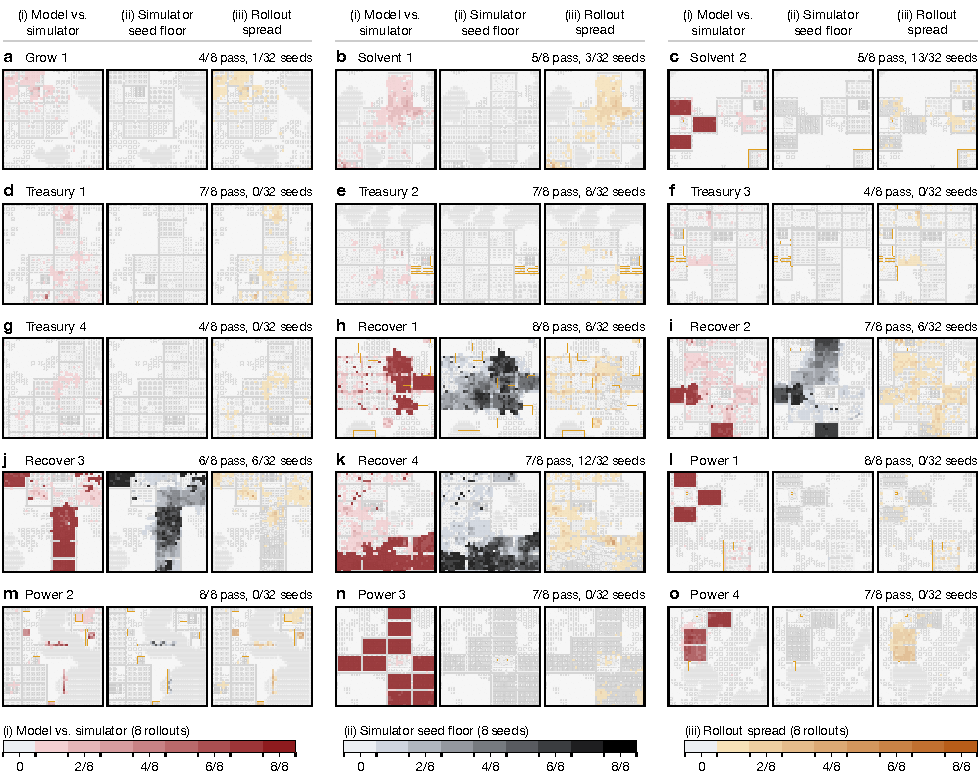
\includegraphics[width=\textwidth]{figures/fig_heatmaps.pdf}
\caption{\textbf{Spatial decomposition of world-model error, simulator stochasticity, and within-model rollout spread.} For each of the \GalPairs{} exploited city plans in Figure~\ref{fig:gallery} (matching panel letters and \GalCrop{}-by-\GalCrop{} spatial windows, overlaid on desaturated month-\Horizon{} procedural city sprites with gold outlines marking the plan's direct spatial build/demolish footprint), three per-tile heat maps show (i) \emph{Model vs.\ simulator} (share of \HeatSamples{} world-model rollouts diverging in tile class or power status from primary engine replay, crimson), (ii) \emph{Simulator seed floor} (share of \HeatSeeds{} independent engine seeds diverging from the primary seed in the exact simulator, charcoal), and (iii) \emph{Rollout spread} (internal disagreement across the \HeatSamples{} world-model rollouts, amber).}
\label{fig:heatmaps}
\end{figure*}
